\documentclass{beamer}

\usepackage{url}
\usepackage{amsmath,amssymb}
\usepackage{graphicx,svg}

\begin{document}
\title{Lecture 2\\ Modeling and Characterization of Signals and Systems}
\author{C.L. Wyatt}
\date{\today}
\maketitle

\begin{frame}
  \frametitle{Introduction}

  Today's lecture is a review of material from ECE 2714. We will review the modeling and characterization of continuous-time and discrete-time signals and systems.

\end{frame}

\begin{frame}
  \frametitle{Signals}

  Signals are modeled as functions $f: A \rightarrow B$ where $A$ and $B$ are sets.

Examples of some commonly encountered signals:

\begin{itemize}
\item
  $A\in \mathbb{R}$, $B\in \mathbb{R}$: CT (Analog) signals
\item
  $A\in \mathbb{Z}$, $B\in \mathbb{R}$: DT real-valued signals
\item
  $A\in \mathbb{Z}$, $B\in \mathbb{C}$: DT complex-valued signals
\item
  $A\in \mathbb{R}$, $B\in \mathbb{R}^2$: two-channel CT (Analog Stereo) signals
\end{itemize}

\end{frame}

\begin{frame}
  \frametitle{Primitive Signals}

  To model signals we can build them up from primitive signals using transformations and combinations.

Some examples of primitive CT signals:

\begin{itemize}
\item
  $\delta(t)$, the delta function
\item
  $u(t)$, the step function
\item
  $e^{st}\; s\in\mathbb{C}$, the complex exponential
\end{itemize}

\end{frame}

\begin{frame}
  \frametitle{Testing Code}

\begin{verbatim}
int x = 3;

// comment
\end{verbatim}

\end{frame}

\begin{frame}
  \frametitle{Testing Images}
  \begin{figure}
    \centering
    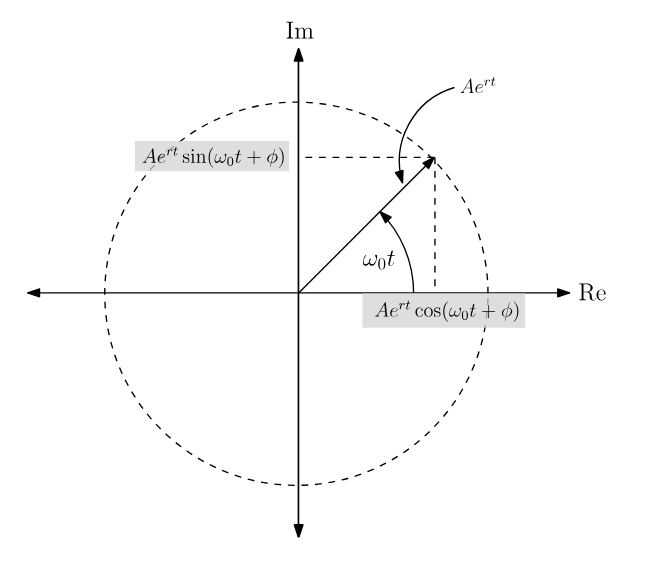
\includegraphics[width=0.4\linewidth, alt={CT complex exponential at one point in time}]{testimage.png}
    \caption{CT complex exponential at one point in time.}
  \end{figure}

\end{frame}

\end{document}
